
\documentclass[11pt]{article}
\usepackage[margin=1in]{geometry}
\usepackage{graphicx}
\usepackage{hyperref}
\usepackage{enumitem}
\usepackage{float}
\usepackage{booktabs}
\usepackage{longtable}
\usepackage{caption}

\title{Axis of Leverage: How China, Pakistan, and India Weaponize Afghanistan’s Weakness}
\author{Ronald J. Botelho}
\date{May 27, 2025}

\begin{document}

\maketitle

\noindent\textit{This article builds on our earlier post titled \textbf{\href{https://ron573.substack.com/p/strategic-engagements-india-pakistan-china-taliban}{Strategic Engagements of India, Pakistan, and China with the Taliban}} (May 25, 2025).}

\section*{Introduction}

In international affairs, weakness is never neutral. It attracts pressure, invites manipulation, and becomes a vessel for someone else’s design. Nowhere is this more visible than in Afghanistan—where three regional powers, once bitterly divided, now circle a fragile regime with calibrated intent.

China builds roads. Pakistan \textbf{builds fences}. India sends aid. All are constructing influence.

This article maps the triangular system of pressure that China, Pakistan, and India exert on Afghanistan—and how the Taliban, often underestimated, has learned to play them off one another in a balancing act more complex than war itself.

\section*{Influence Map}

\begin{figure}[H]
\centering
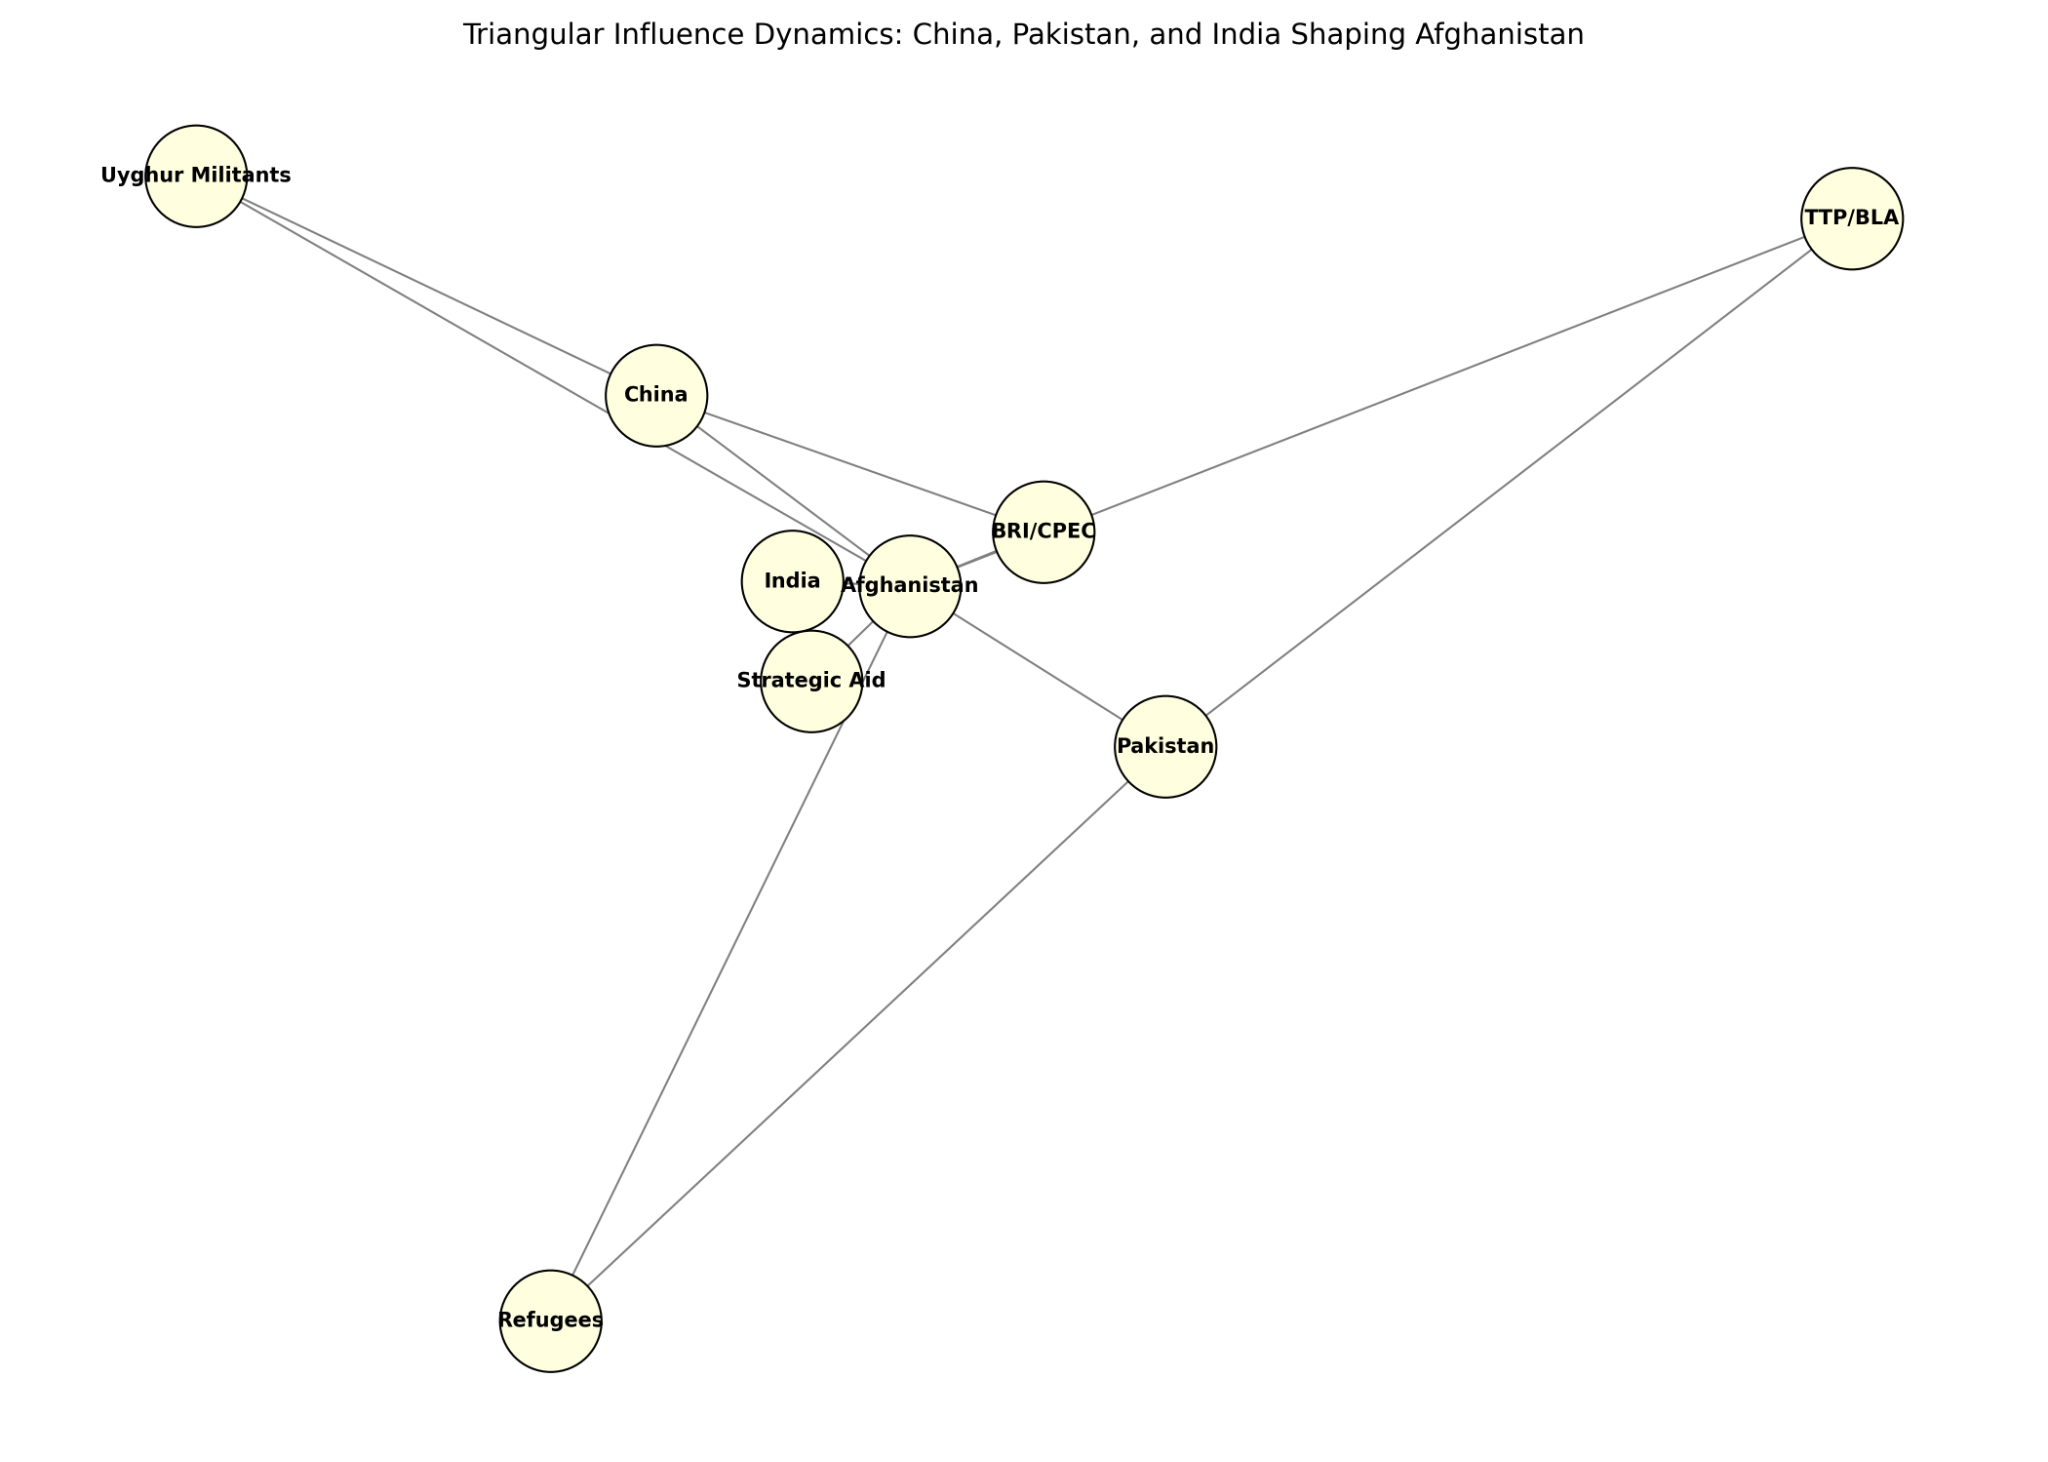
\includegraphics[width=0.9\textwidth]{axis_of_leverage_map.png}
\caption*{Left: Triangular Influence Dynamics (Botelho, 2025)}
\end{figure}

\begin{figure}[H]
\centering
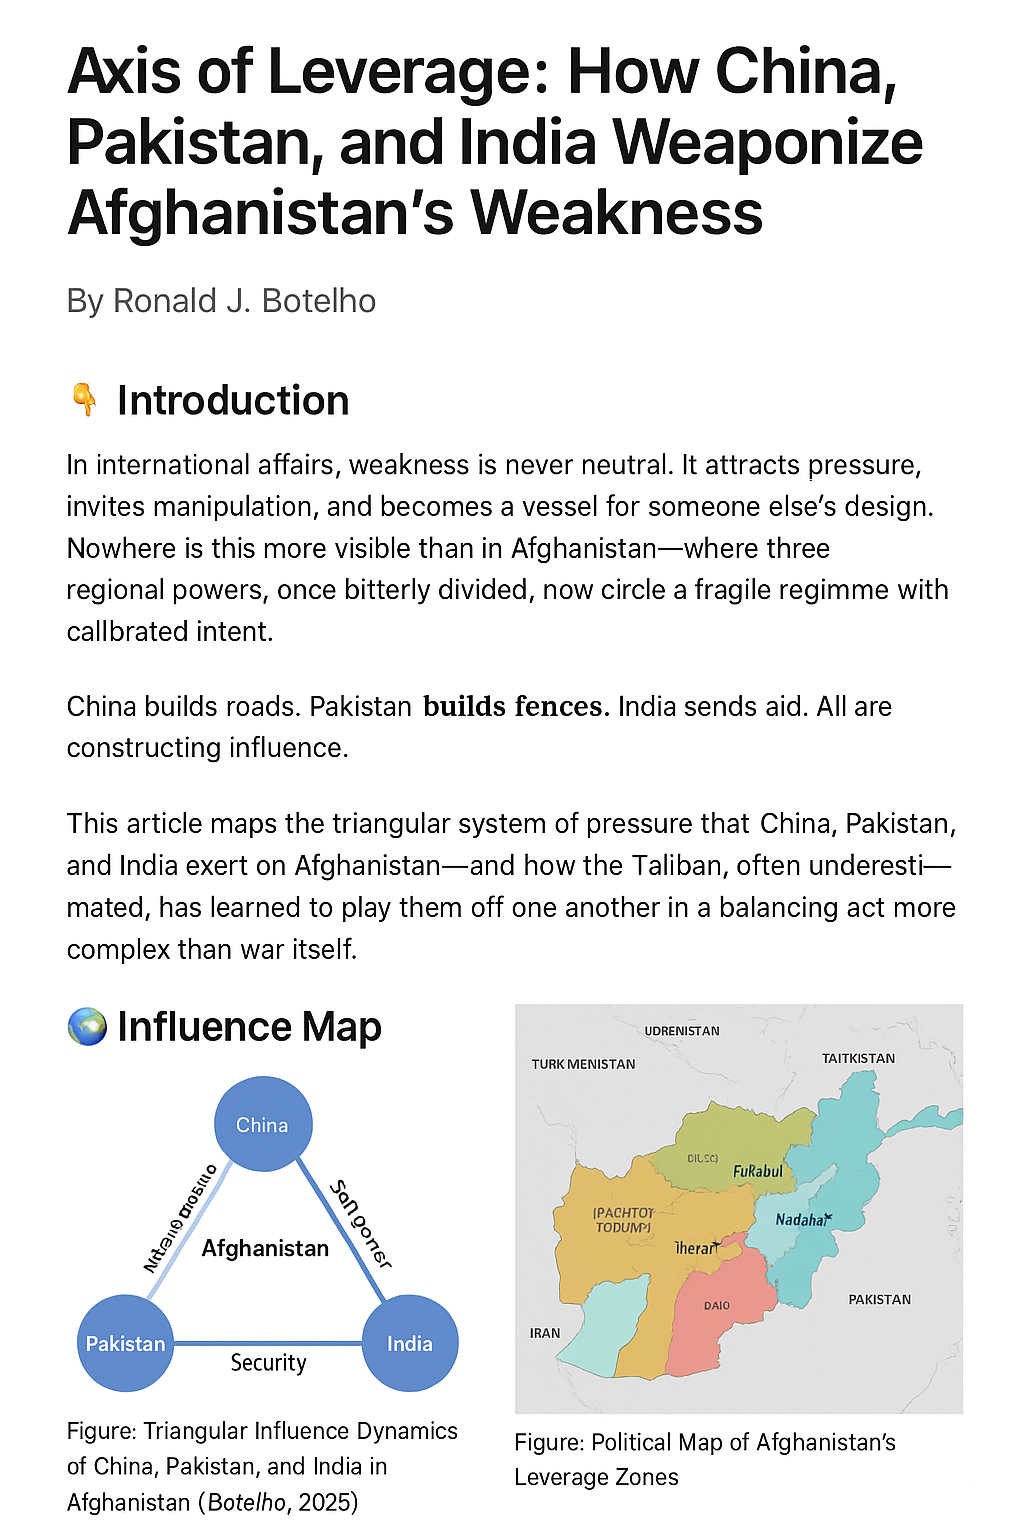
\includegraphics[width=0.9\textwidth]{afghan_ethnolinguistic_map.png}
\caption*{Right: Political Map of Afghanistan’s Leverage Zones (2025)}
\end{figure}

\section*{Ethnolinguistic and Territorial Overview}

Afghanistan remains a fractured state in both language and identity. The Taliban draws its power base from southern Pashtun tribes, while resistance groups and traditional power brokers operate in Dari-speaking central highlands and Uzbek-speaking northern provinces. This ethnolinguistic segmentation complicates any single power's ability to project cohesive control, allowing external actors like China, Pakistan, and India to form regionally selective alliances.

\section*{Structural Overview}

Afghanistan is the pivot point in a pressure triangle formed by China, Pakistan, and India. Each actor deploys a distinct strategy: infrastructure, security, and soft power.

\subsection*{Actor-by-Actor Analysis}

\textbf{China} Objectives: Secure Belt and Road expansion, mineral access, Xinjiang buffer (Zhou, 2024). Tactics: Recognize Taliban diplomats, invest in mining, integrate Afghanistan into CPEC.\\
\textbf{Pakistan} Objectives: Contain TTP and BLA, control refugee flows, preserve Kabul influence (Khan, 2023). Tactics: Forced deportations, border military pressure, back-channel Taliban negotiations.\\
\textbf{India} Objectives: Counter China-Pakistan axis, secure trade routes, maintain goodwill (Mehta, 2023). Tactics: Humanitarian aid, quiet diplomacy, investment in Chabahar.\\
\textbf{Afghanistan} Objectives: Achieve regime legitimacy, secure foreign investment, preserve sovereignty, and leverage transient geopolitical rivalries (Rahimi, 2024). Tactics: Sell recognition, export instability, and negotiate tactical concessions.

\section*{Strategic Posture of Regional Powers}

\begin{longtable}{|p{2.5cm}|p{4.5cm}|p{4.5cm}|p{4.5cm}|}
\hline
\textbf{Country} & \textbf{Strategic Objectives} & \textbf{Tactics} & \textbf{Core Interests} \\
\hline
\endfirsthead
\hline
\textbf{Country} & \textbf{Strategic Objectives} & \textbf{Tactics} & \textbf{Core Interests} \\
\hline
\endhead

\textbf{China} &
\begin{itemize}[leftmargin=*]
\item Expand BRI and CPEC
\item Secure Xinjiang buffer
\item Access mineral wealth
\end{itemize} &
\begin{itemize}[leftmargin=*]
\item Recognize Taliban diplomats
\item Mining deals
\item Infrastructure investment
\end{itemize} &
\begin{itemize}[leftmargin=*]
\item Economic corridors
\item Security in West China
\end{itemize} \\
\hline

\textbf{Pakistan} &
\begin{itemize}[leftmargin=*]
\item Control TTP/BLA spillover
\item Reassert Afghan influence
\item Deport refugees
\end{itemize} &
\begin{itemize}[leftmargin=*]
\item Border fencing
\item Mass deportations
\item Back-channel talks
\end{itemize} &
\begin{itemize}[leftmargin=*]
\item Strategic depth
\item Internal security
\end{itemize} \\
\hline

\textbf{India} &
\begin{itemize}[leftmargin=*]
\item Counterbalance China-Pakistan axis
\item Secure trade routes
\item Project regional soft power
\end{itemize} &
\begin{itemize}[leftmargin=*]
\item Humanitarian aid
\item Quiet diplomacy
\item Investment in Chabahar
\end{itemize} &
\begin{itemize}[leftmargin=*]
\item Trade access
\item Regional leverage
\end{itemize} \\
\hline

\textbf{Afghanistan} &
\begin{itemize}[leftmargin=*]
\item Leverage international rivalries
\item Consolidate Taliban control
\item Attract foreign aid
\end{itemize} &
\begin{itemize}[leftmargin=*]
\item Play powers against one another
\item Sell recognition
\item Exploit instability
\end{itemize} &
\begin{itemize}[leftmargin=*]
\item Political legitimacy
\item Regime survival
\end{itemize} \\
\hline
\end{longtable}

\section*{Actor Interactions and Intelligence Influence}

\begin{figure}[H]
\centering
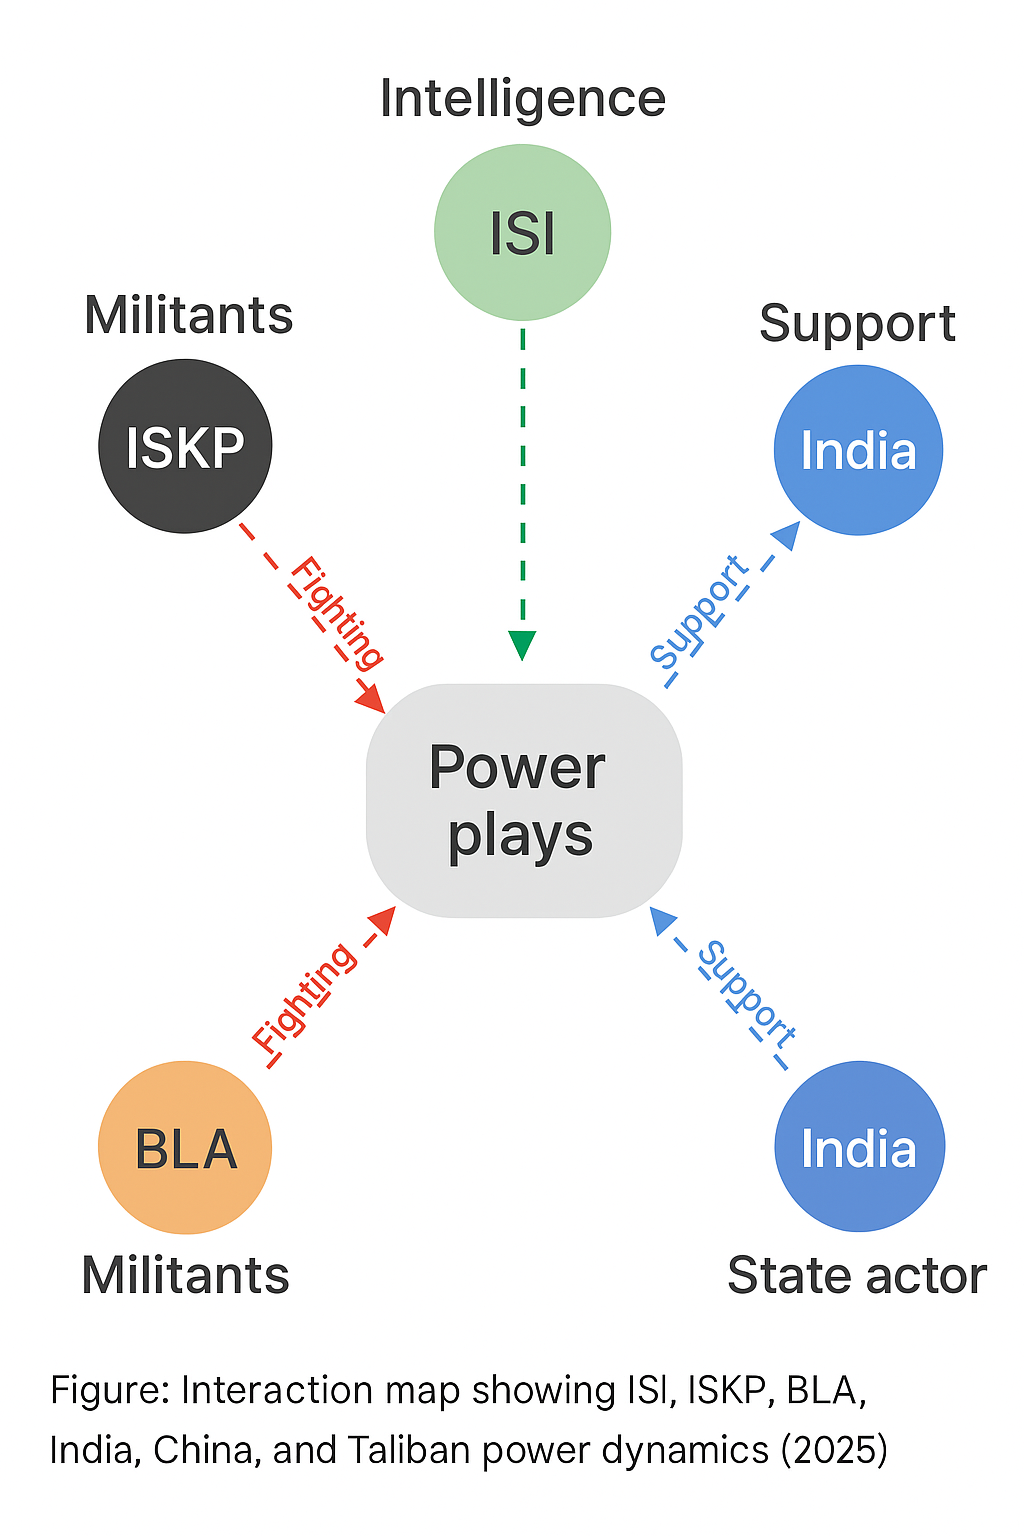
\includegraphics[width=0.9\textwidth]{fragmetation_and_power-plays.png}
\caption*{Militant and Intelligence Interaction Map: ISI, ISKP, BLA, India, and Taliban (2025)}
\end{figure}

\section*{Feedback Loops and Risks}

\begin{figure}[H]
\centering
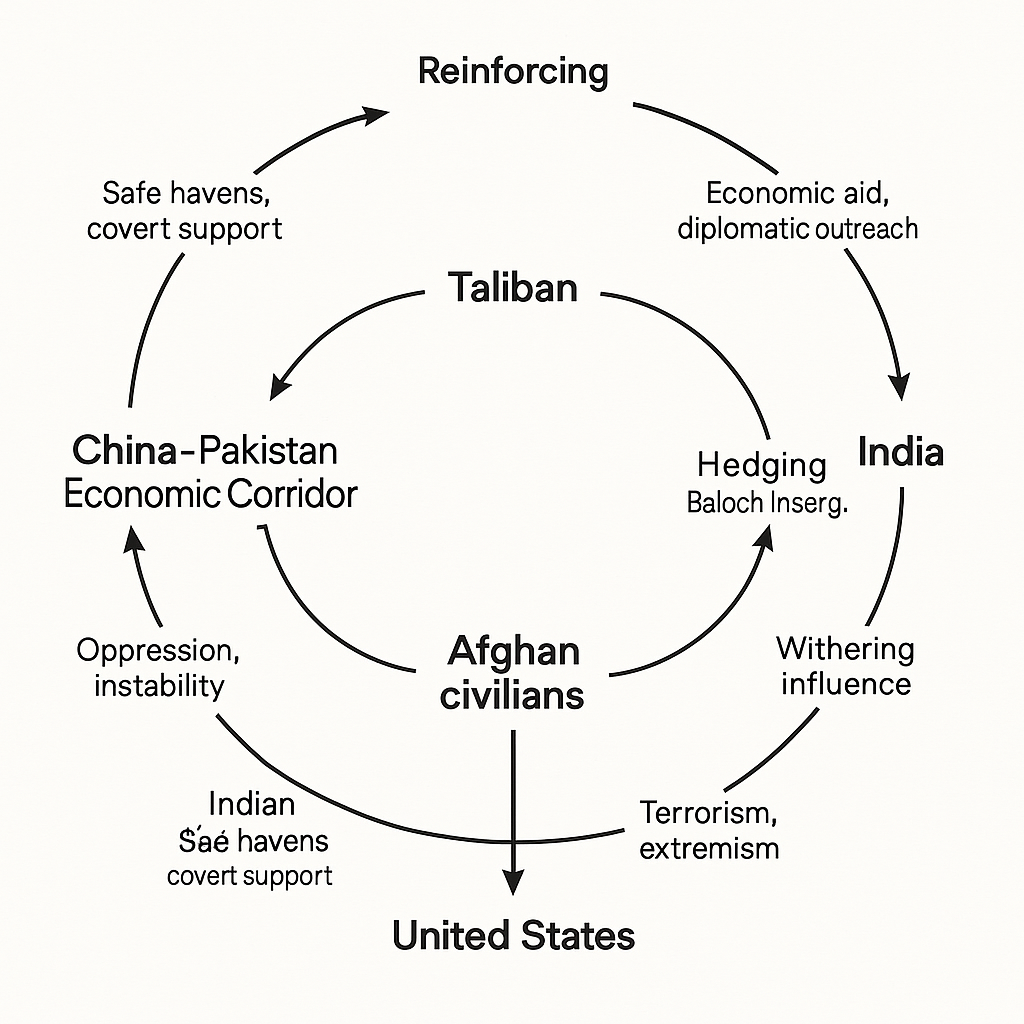
\includegraphics[width=0.9\textwidth]{strategic_feedback.png}
\caption*{Feedback dynamics showing how recognition, aid, and regional pressure fuel Taliban consolidation (2025)}
\end{figure}

\section*{Strategic Scenarios}

\begin{itemize}
\item \textbf{Stability Deal}: Multilateral investment stabilizes region. Beneficiaries: China, Taliban
\item \textbf{Controlled Collapse}: Instability maintains strategic ambiguity. Beneficiaries: Taliban, Pakistan
\item \textbf{Proxy Spiral}: Escalating rivalries push region toward armed conflict. Beneficiaries: None; India at risk
\end{itemize}

\section*{References}

Ghosh, P. (2023). \textit{South Asia’s proxy politics and the Afghan vacuum}. Observer Research Foundation.\\
Khan, I. (2023). \textit{Pakistan’s refugee strategy and the Taliban}. Dawn News. \url{https://www.dawn.com}\\
Mehta, S. (2023). \textit{India’s emerging diplomacy with Taliban}. Indian Express. \url{https://www.indianexpress.com}\\
Rahimi, T. (2024). \textit{Taliban's leverage in regional multipolarity}. Afghan Institute for Strategic Studies (AISS).\\
Zhou, Y. (2024). \textit{China’s frontier doctrine and BRI’s western edge}. Journal of Geopolitical Strategy.

\section*{Disclaimer}
The views expressed are solely those of the author, Ronald J. Botelho, a Ph.D. student in Complex Sciences at Binghamton University. This article is for academic and public analysis purposes only.

\section*{Disclosure}
Visuals and code for the influence map can be found at: \url{https://github.com/Ron573/substack-archive}

\end{document}
